% !TEX root = poster.tex
\headerbox{\textbf{Flavour Tagging in Run I}}{name=run1,column=1,span=2,row=0}{
\begin{minipage}{0.474\boxwidth}
\textbf{Strategy}\\[-0.85em]
\begin{itemize}
\setlength\itemsep{0.01em}
\vspace{-0.3em}
\item for each tagger one calibration valid for all channels 
\item systematic uncertainties from
\begin{itemize}
\setlength\itemsep{0.01em}
\setlength{\itemindent}{-.11in}
\vspace{-0.4em}
\item[${\color{tu_gruen}-}$] calibration methods
\item[${\color{tu_gruen}-}$] results in different control channels 
\end{itemize}
\vspace{-0.4em}
\item "ad-hoc" calibration from specific control channels for analyses dominated by FT uncertainty %(\BdToJPsiKS)
\end{itemize}
\vspace{-0.9em}
%\begin{center}
%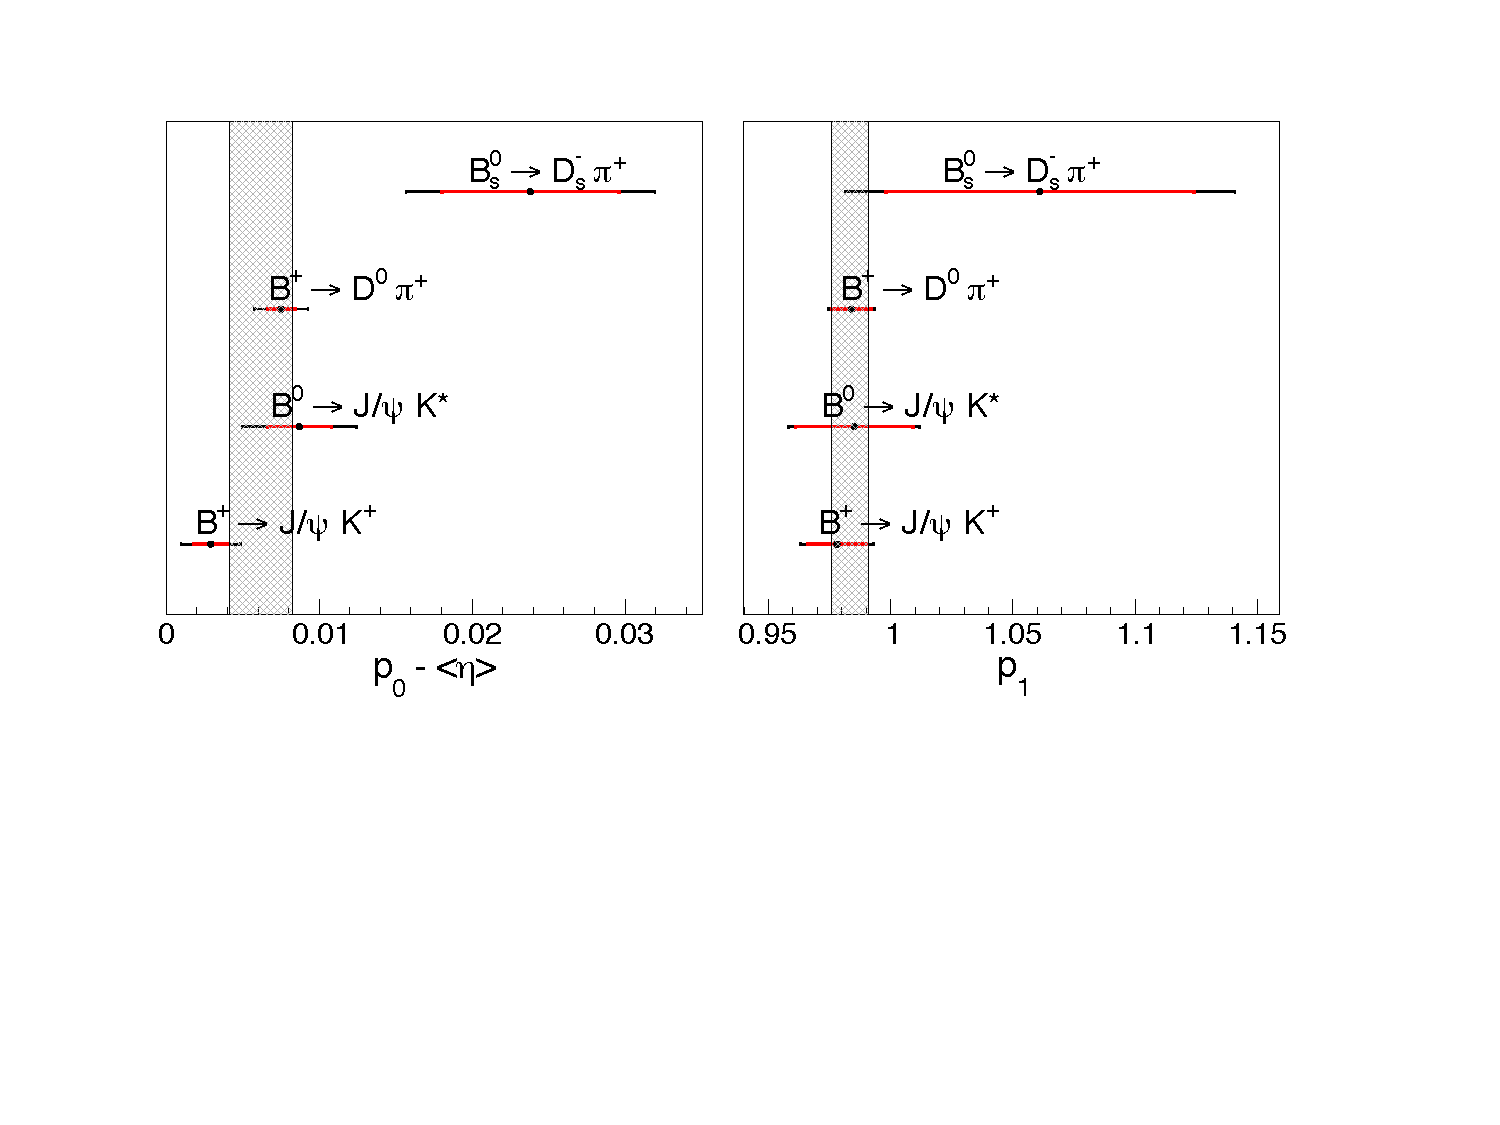
\includegraphics[width=0.466\boxwidth]{graphP0P1.pdf}
%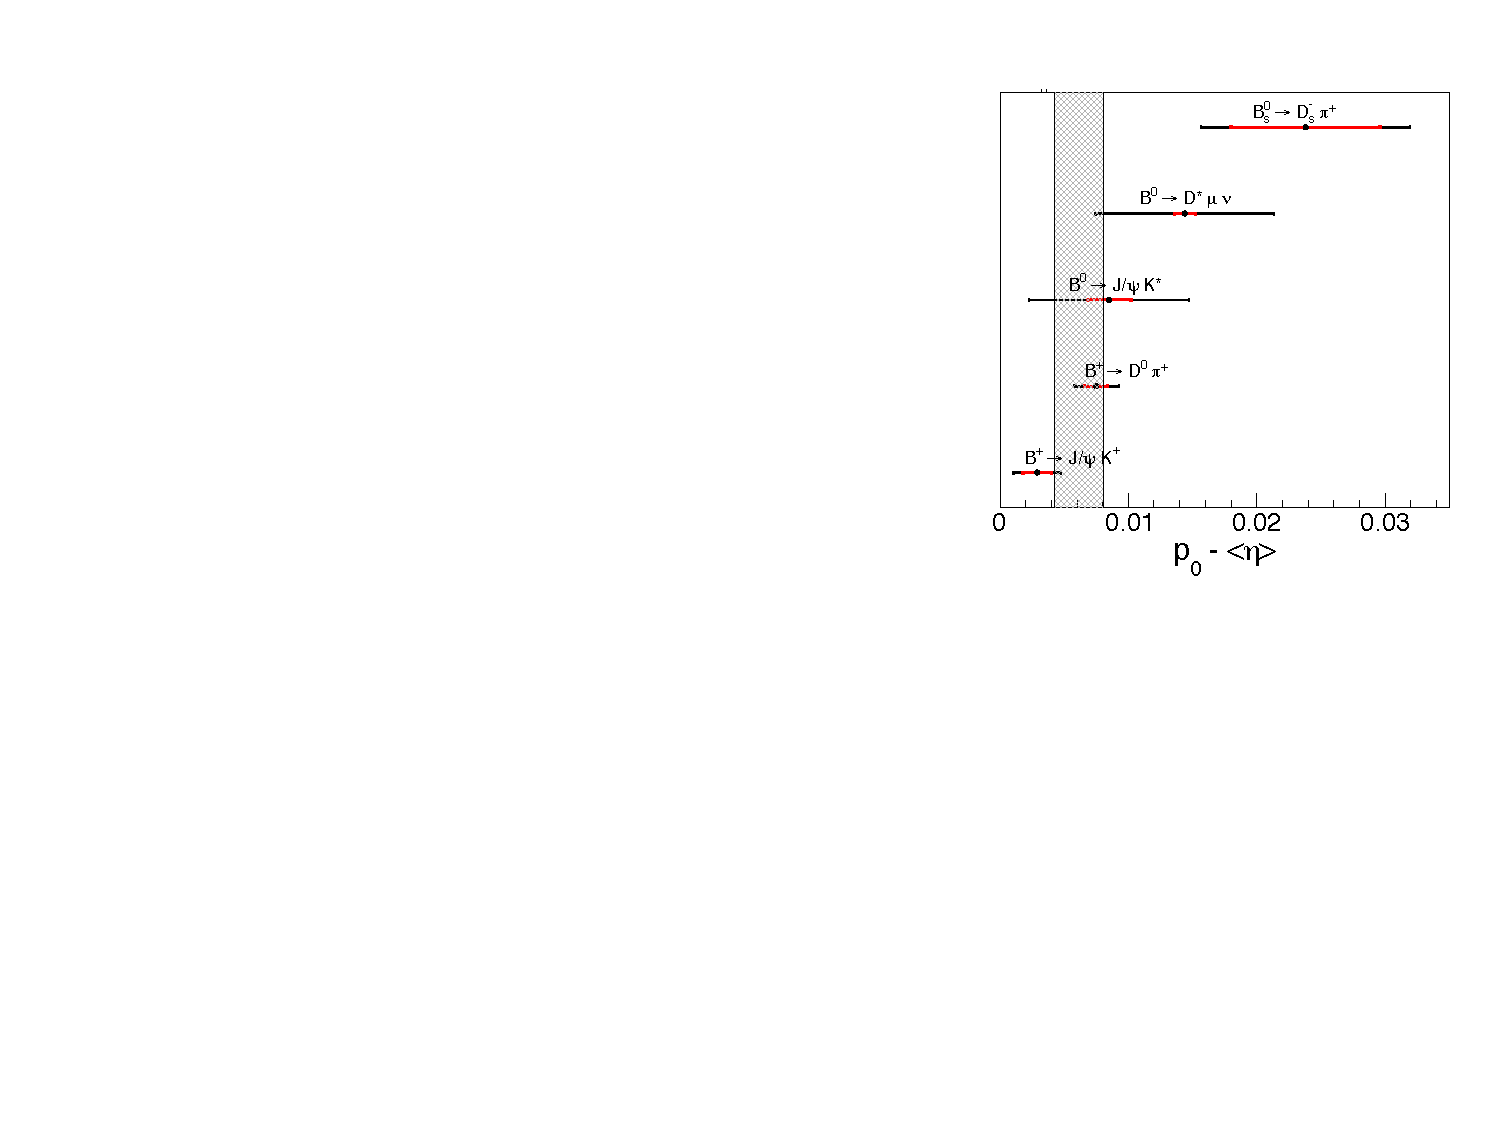
\includegraphics[width=0.233\boxwidth]{portability_p0.pdf}
%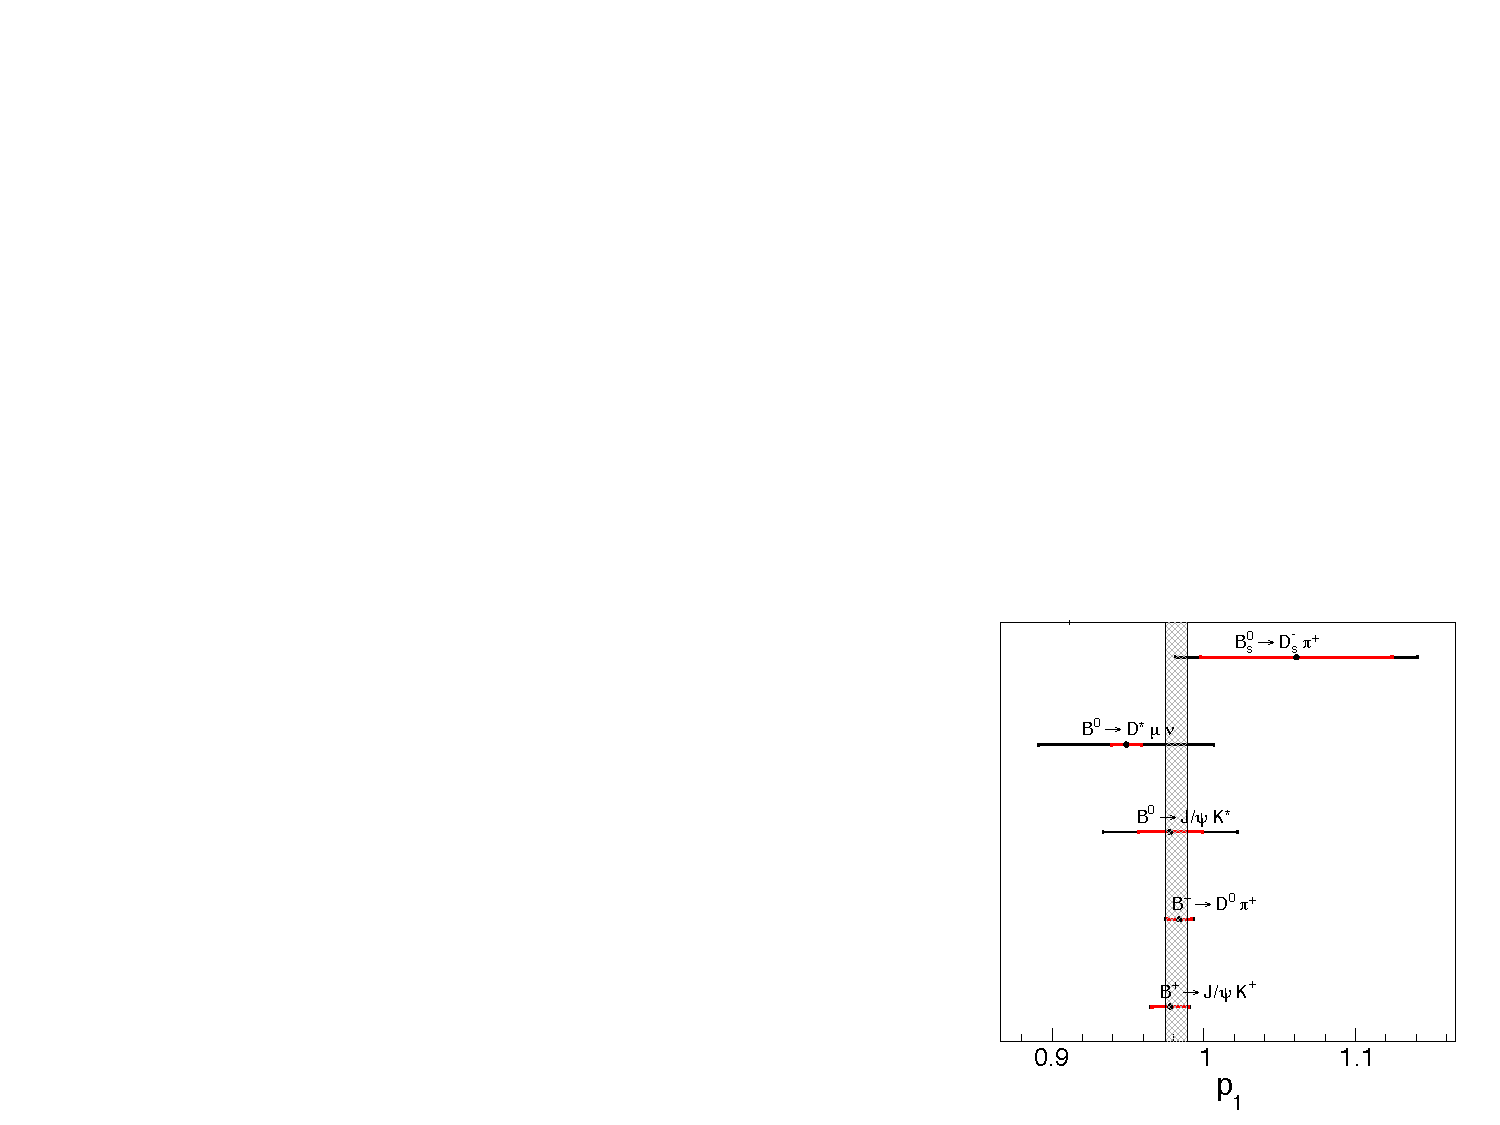
\includegraphics[width=0.233\boxwidth]{portability_p1.pdf}
%\end{center}
\vspace{1.15em}
\textbf{Performance in analyses}
\vspace{-0.5em}
\begin{itemize}
\item\textbf{CP violation in \BsToJPsipipi}

\vspace{-1.7em}
\begin{center}
\includegraphics[width=0.315\boxwidth]{figures/Jpsipipi_SSK.pdf}
\end{center}
\vspace{-2.7em}

	\begin{itemize}
	\setlength\itemsep{0.01em}
	\setlength{\itemindent}{-.11in}
	\item[${\color{tu_gruen}-}$] two analyses:
	\setlength{\itemindent}{.05in}
	\item[${\color{tu_gruen}\rightarrow}$] on \SI{1}{\invfb}: $\varepsilon_\text{eff}=\SI{2.43}{\%}$ [3] 
	\item[${\color{tu_gruen}\rightarrow}$] on  \SI{3}{\invfb}: $\varepsilon_\text{eff}=\SI{3.89}{\%}$ [4]
	\setlength{\itemindent}{-.11in}
	\item[${\color{tu_gruen}-}$] second analysis included SS kaon nnet tagger
	\item[${\color{tu_gruen}-}$] OS algorithms have been re-optimised
	\end{itemize}
	
\item\textbf{CP violation in \BsToDsK}

\vspace{-1.7em}
\begin{flushleft}
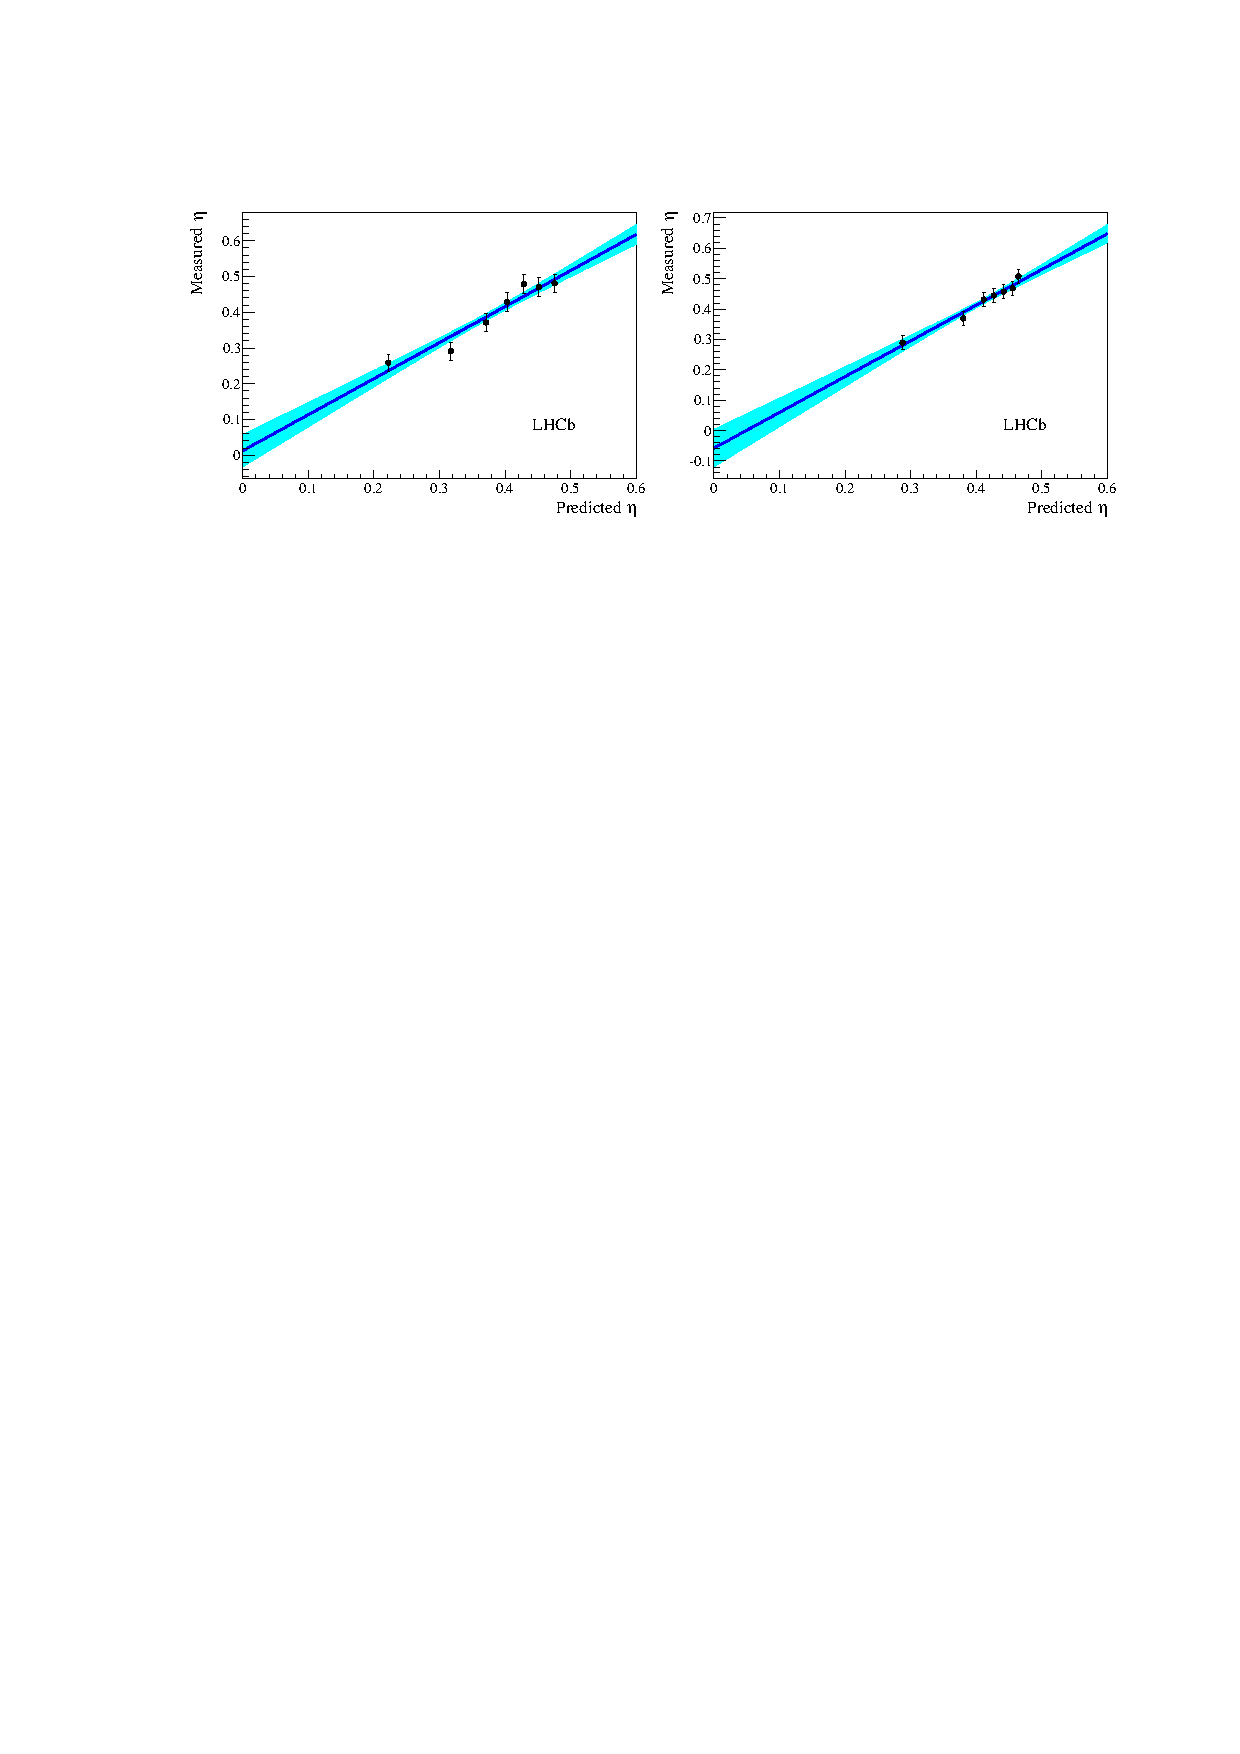
\includegraphics[width=0.474\boxwidth]{CPV_DsK1.pdf}
\end{flushleft}
\vspace{-2.5em}

	\begin{itemize}
	\setlength\itemsep{0.01em}
	\setlength{\itemindent}{-.11in}
	\item[${\color{tu_gruen}-}$] SS kaon nnet (right) adds more than \SI{1.3}{\%} to $\varepsilon_\text{eff}$ (OS calibration left) [5]
	\end{itemize}
\end{itemize}
\end{minipage}
\vspace{0.7em}
\hfill
\begin{minipage}{0.474\boxwidth}
\vspace{-1.2em}
\begin{itemize}
\item\textbf{CP violation in \BdToJPsiKS ($\sin2\beta$)}
	\begin{itemize}
	\setlength\itemsep{0.01em}
	\setlength{\itemindent}{-.11in}
	\item[${\color{tu_gruen}-}$] compared to the \SI{1}{\invfb} analysis the SS pion tagger adds more than \SI{0.376}{\%} to $\varepsilon_\text{eff}$ in the\SI{3}{\invfb} analysis
	\item[${\color{tu_gruen}-}$] precision analysis \hspace{0.1em}${\color{tu_gruen}\rightarrow}$ "ad-hoc" calibration with \BuToJPsiKp (OS) and \BdToJPsiKst (SS pion) leads to smaller uncertainties from FT [6]
	\end{itemize}

\vspace{-1.7em}
\begin{center}
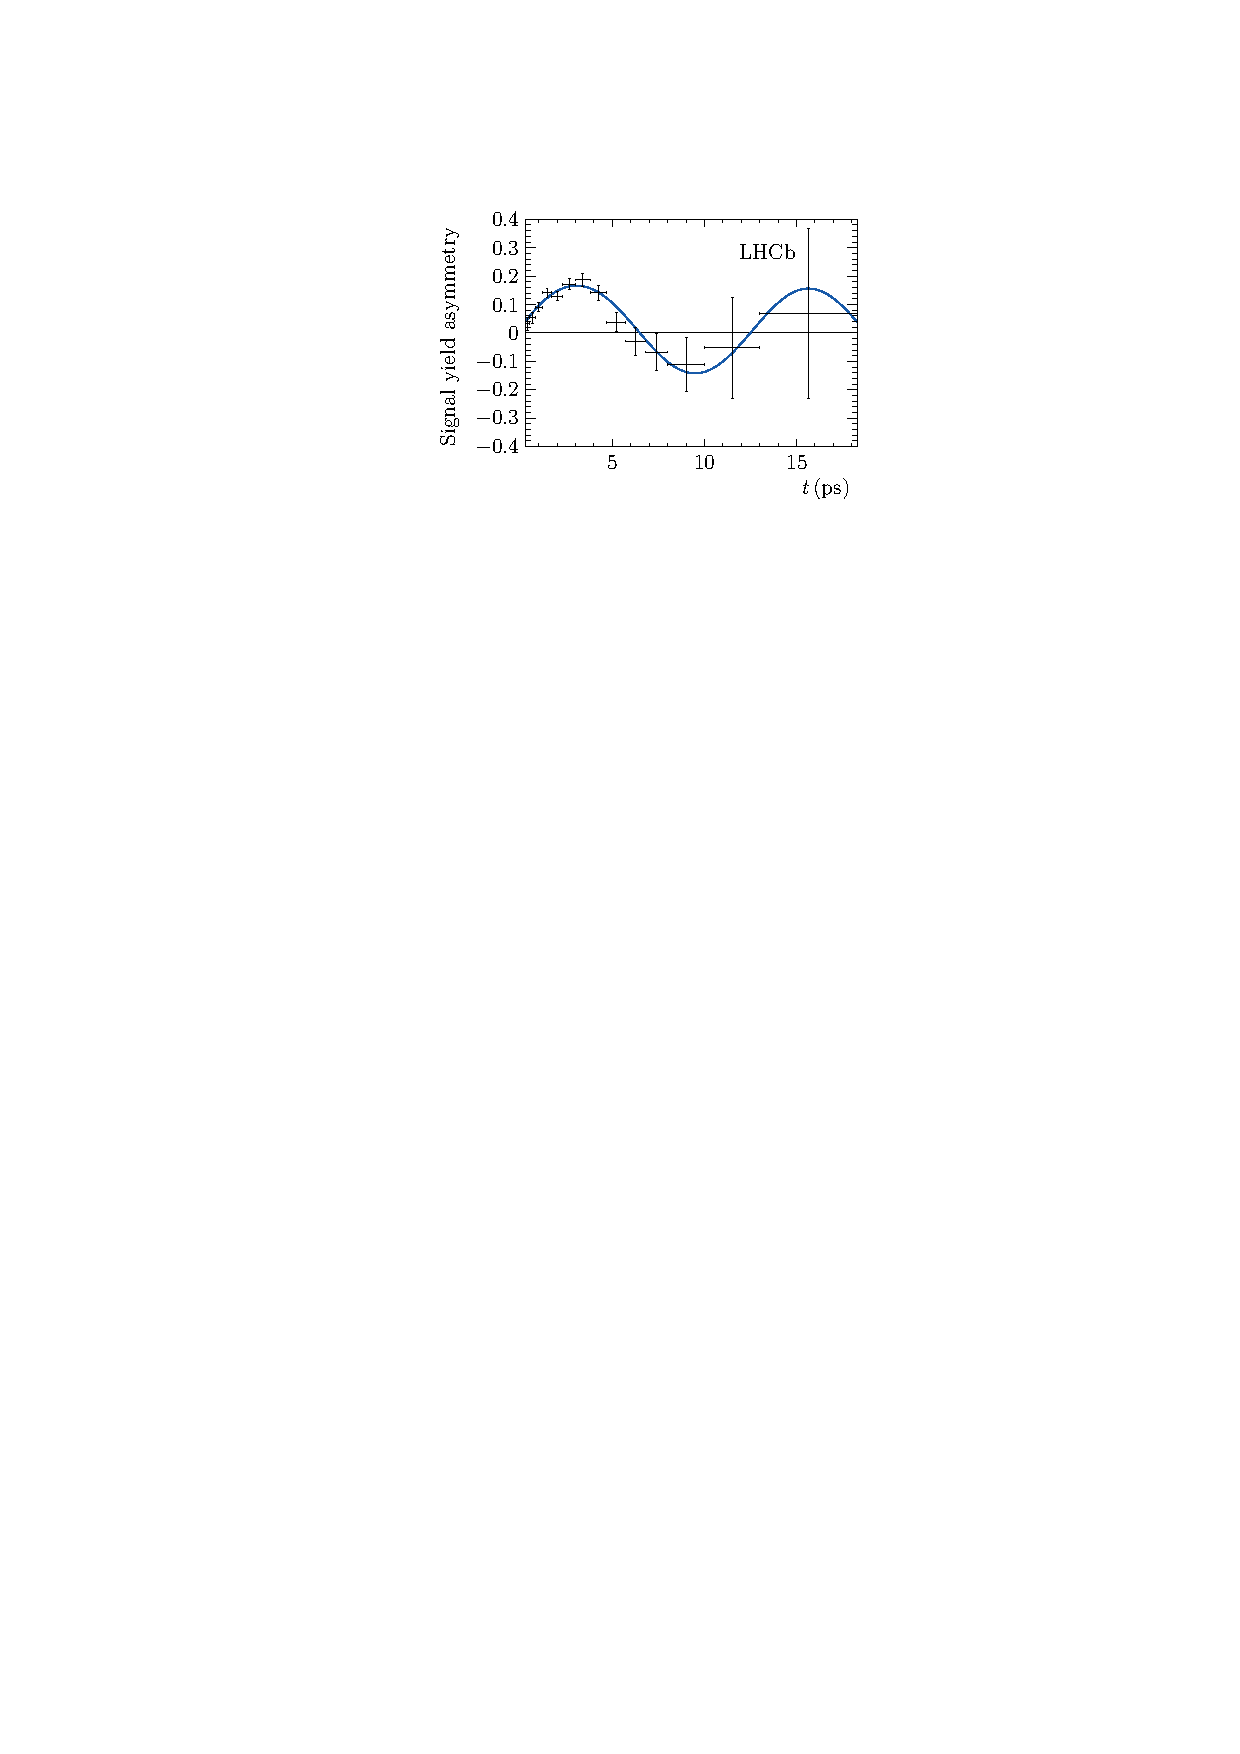
\includegraphics[width=0.315\boxwidth]{CPV_sin2beta.pdf}
\end{center}
\vspace{-2.5em}

%\item\textbf{\BsTophiphi}

\item\textbf{CP violation in \BsToJPsiKS}
	\begin{itemize}
	\setlength\itemsep{0.01em}
	\setlength{\itemindent}{-.11in}
	\item[${\color{tu_gruen}-}$] \Bs and \Bd events not separable in analysis
	\item[${\color{tu_gruen}-}$] \Bs events: $\varepsilon_\text{eff}=\SI{4.00}{\%}$ [7]
	\item[${\color{tu_gruen}-}$] \Bd events: also small contribution of SS kaon to $\varepsilon_\text{eff}$
	\setlength{\itemindent}{.05in}
	\item[${\color{tu_gruen}\rightarrow}$] same-side protons misidentified as kaons
	\item[${\color{tu_gruen}\rightarrow}$] kaons from \Kstar(892) produced in correlation with the \Bz
	\item[${\color{tu_gruen}\Rightarrow}$] kaons have charge opposite: tag decision has to be inverted
	\end{itemize}
%\item\textbf{Measurement of \dms with \BsToDspi}
%
%\vspace{-1.7em}
%\begin{center}
%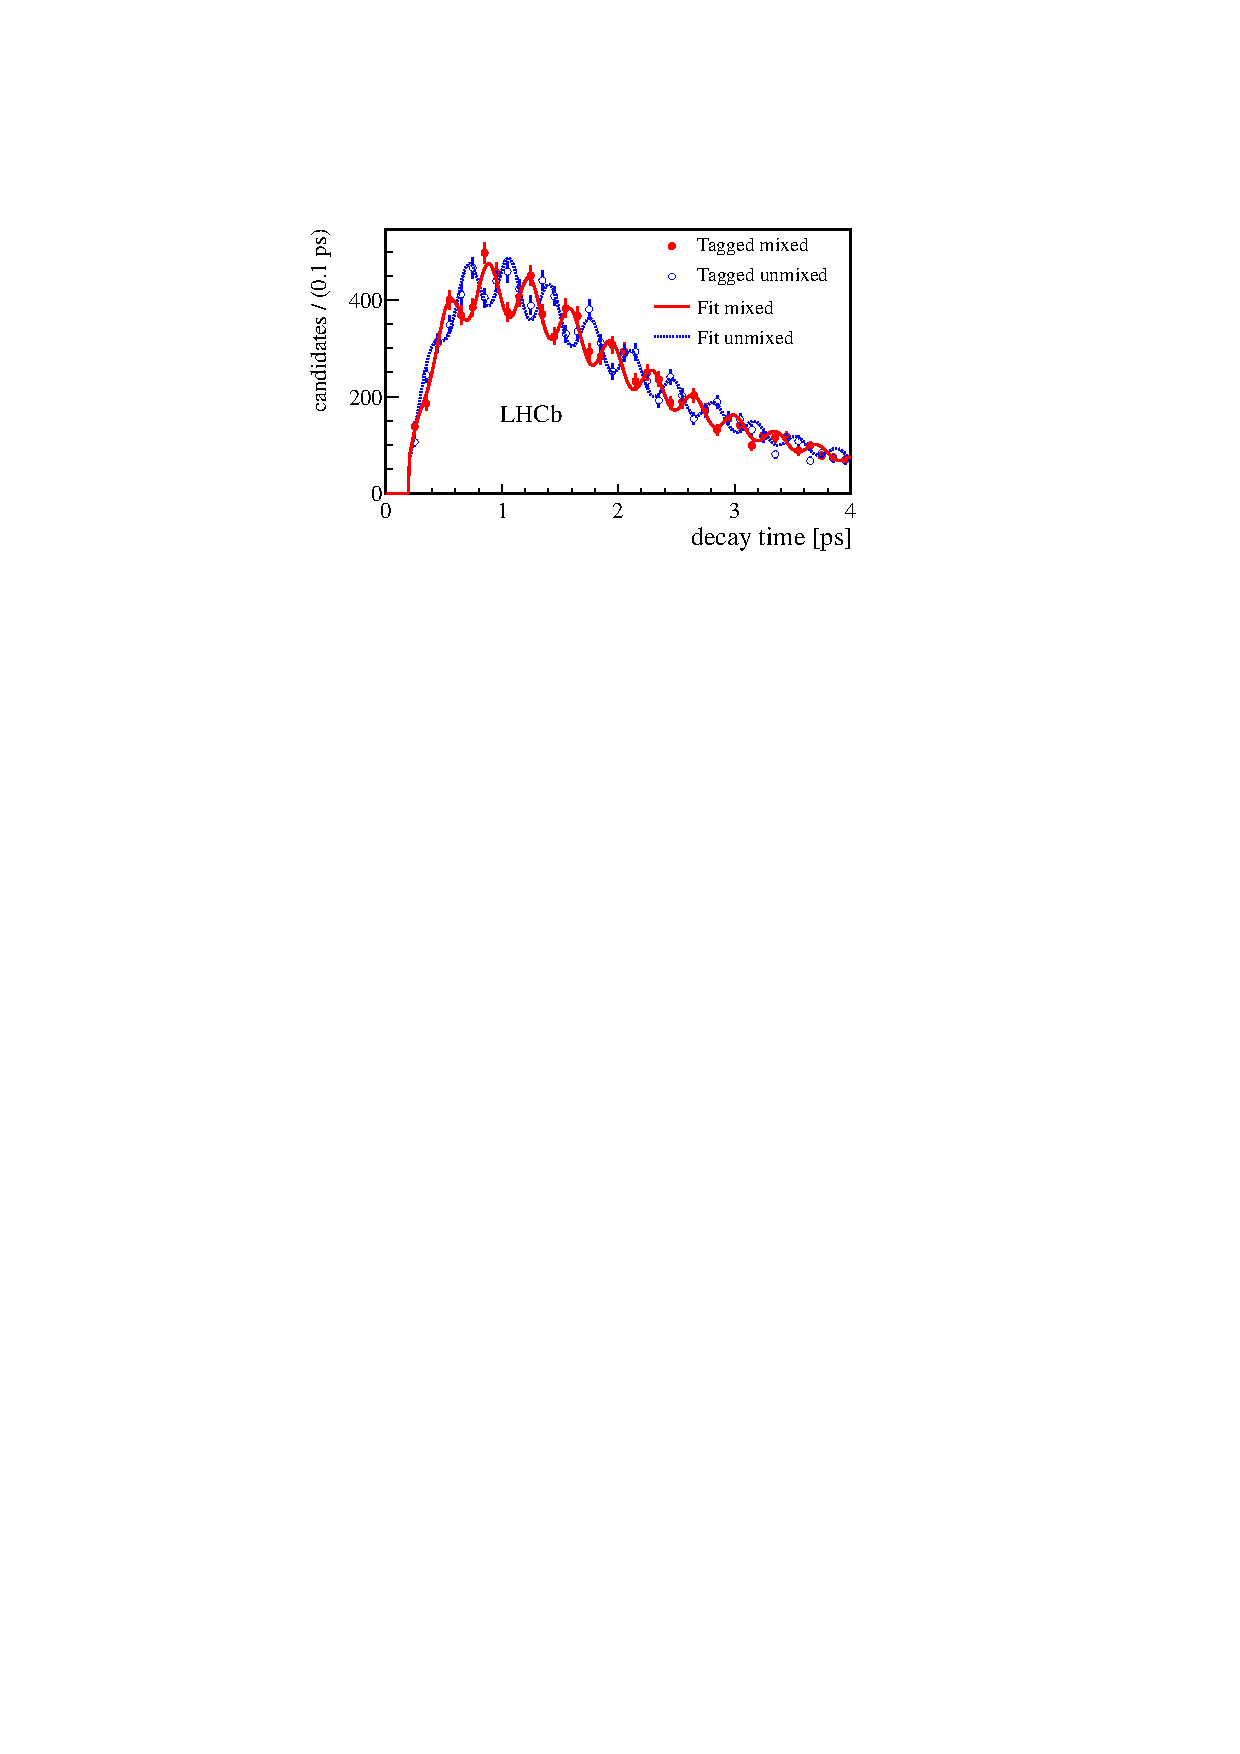
\includegraphics[width=0.266\boxwidth]{Bs_mixing1.pdf}
%\end{center}
%\vspace{-2.5em}
%
%	\begin{itemize}
%	\item[${\color{tu_gruen}-}$] Decay rates: $e^{-\Gamma t}\left(...+\!d\cos\left(\Delta mt\right)\right)$
%	\end{itemize}
\end{itemize}

\textbf{Overall performance improvements in Run I}
\begin{itemize}
\setlength\itemsep{0.01em}
\vspace{-0.3em}
\item OS tagging improved $\mathcal{O}$(15\%) 
\item SS kaon tagging improved $\mathcal{O}$(40\%)
\vspace{0.5em}
\setlength{\itemindent}{.14in}
\item[$\color{tu_gruen}\Rightarrow$] \textbf{Flavour Tagging has been a success in Run I}
\end{itemize}
\end{minipage}
\vspace{-0.5em}
}
